\documentclass[11pt]{article}
\usepackage{iitbtitle}
\usepackage{caption}
\usepackage{subcaption}
\usepackage{a4wide}
\usepackage{multirow} 
\usepackage{anysize}
\usepackage{iitbcs}
\usepackage{latexsym}
\usepackage{amssymb}
\usepackage{amsmath}
\usepackage{graphicx}
\usepackage{epsfig}
\usepackage{comment}
% \usepackage{psfig}
\usepackage{tabls}
\usepackage{multirow}
\usepackage{tabularx}
\usepackage{url}
\newcolumntype{Y}{>{\centering\arraybackslash}X}
\setlength{\floatsep}{7pt plus 2pt minus 2pt}
\setlength{\textfloatsep}{5pt plus 2pt minus 2pt}
\setlength{\intextsep}{5pt plus 2pt minus 2pt}
\usepackage{color}

\marginsize{2.5cm}{2.5cm}{1cm}{1.5cm}
\def\baselinestretch{1.15}

\newcommand\INPUT{\item[\textbf{Input:}]}
\newcommand\OUTPUT{\item[\textbf{Output:}]}
\providecommand{\norm}[1]{\lVert#1\rVert}
\DeclareGraphicsExtensions{.pdf,.png,.jpg}
\begin{document}


%\baselineskip 20pt
%The definitions
\def\title{Quadcopter Based Applications in Imaging}
\def\what{Third Annual Progress Report}
\def\degree{Doctor of Philosophy}
\def\who{Meghshyam G. Prasad}
\def\roll{124058001}
\def\guide{Prof. Sharat Chandran \\ Prof. Michael Brown}
\titlpage
\def\bsq{\begin{flushright} $\blacksquare$\\ \end{flushright}}
\def\tab{\hspace{5mm}}

\newpage
\section*{Acknowledgements}
I express deep and sincere gratitude to Prof. Sharat Chandran and Prof.
Michael Brown for providing constant direction and guidance. I am also
very much grateful to Prof. David Hsu for giving me access to his lab and
equipments. I am also thankful to Mr. Abhishek Chakrborty and Mr. Ravi Chalasani
for their help in stangnant water detection project.

\begin{flushright}
Meghshyam G. Prasad
\end{flushright}

\pagenumbering{roman}
\newpage
\begin{abstract}
In today's world, digital imaging is being extensively used in almost all
sectors. In some situations, it is quite difficult to take pictures from
handheld camera. Low cost quadcopters such as Parrot's AR Drone may be used in
such scenarios to take photos of an object which is otherwise out of reach of normal
camera. There are two problems involved in it: first to track the given object
and second to take ``good'' pictures of it. In my last APS we discussed 
about the first problem. Here, we will see how to take good pictures and use it for
variouos applications.

One of the use case where we may use quadcopter for imaging is to
capture a panaroma of big wall (or any such planar object). In such cases, it
will be very tedious and tiring to use hand held camera. Secondly, if there are
vacant spaces on a wall, it is challenging for existing mosaicing techniques as
there will be little to no features to match input images. So, in our work, we
focuses on a method to construct panoramas captured from a quadcopter, that
consists of scenes with significant regions of vacant spaces.

We describe a framework that is able to handle this unique input by
leveraging the availability of the inertial measurement unit (IMU)
data from the quadcopter that is synchronized with the input images.
We use the IMU data for two purposes: first to select images which can
be stiched together. Second, in combination with coarse stereo reconstruction,
we determine appropriate portions of the images to complete the panorama. We
demonstrate the efficacy of our approach on a number of input sequences that
cannot to be mosaiced by existing methods.

After using quadcopter for mosaicing of images, we thought of using it for 
some ``survey'' application. In recent times, there has been a sharp increase
in dengue and malaria, especially in urban areas. One of the major reasons for
this health hazard is the number of locations where one can find stagnant
water. These locations are large breeding ground for fast multiplying
mosquitoes, and other insects. Areas include traditionally uncovered gutters,
and also terraces of high rise buildings, and shades above windows (popularly
known as chhajja)-- areas that are hard to reach and access. We propose the use
of a quadcopter to inspect areas and identify stagnant water patches.  Water
being specular in nature tends to confound traditional image processing
methods. Further the use of a non-traditional camera mounted on a quadcopter
presents new challenges.  We provide methods to get past such hurdles.

\noindent \textbf{Keywords:} Quadcopter, Panoramic Image Stitching, Stagnant Water Detection

\end{abstract}
\newpage
\pagenumbering{arabic}
\tableofcontents

%\begingroup\def\thispagestyle#1{}\def\baselinestretch{1.5}\tableofcontents\endgroup
\newpage

\section{Introduction}

\section{Mosaicing Scenes with Vacant Spaces}

Finding features and using them to align images to construct wide field
of view panoramas is one of the success stories of
computer vision.  Virtually all recent consumer cameras have this
technology embedded.  The success of these methods relies significantly on
finding common features in the images that can be used to established the
 appropriate warps to register the images together.

There are scenes, however, that consist of image content that makes this
challenging.  One situation is when scene patterns and texture are repeated.  
This can make it challenging for matching algorithm to find appropriate matches.
A more serious situation is when a scene area simply
does not contain features.  This sort of situation occurs in a variety
of situations such as paintings in an art exhibition, or posters in an
auditorium.

{\bf Key Idea} We propose to solve the vacant space problem by using
an inexpensive off-the-shelf flying device, such as a quadcopter which
can be assumed to contain an inertial measurement unit (IMU) that has
positional information time synchronized with an input video.  The
proximity relationship that the resultant images have, can be used to
significantly reduce the search space in finding matches.  Further,
the proximity relationship also allows, in principle, to vary the
parameters involved in feature selection. For example, if there is
reason to believe that two images are adjacent horizontally, one can
choose to adjust thresholds in feature matching algorithm to hunt for
otherwise elusive matching pairs.

We note that positions can be also made available in other devices
such as smartphones.  An autonomous programmed quadcopter, however, is
particularly enticing because of its ability to fly to areas that are
accessible to the human eye, but inaccessible for the
human to reach.  Such areas do not lend themselves easily to high
quality images.

\subsection{Related Work}
Panoramic image stitching (alternatively, image mosaicing) is a
well-studied problem in the field of computer vision.  Representative
works include~\cite{Milgram1975}, \cite{Milgram1977}, \cite{Capel},
\cite{Szeliski1997} \cite{Brown07} \cite{Brown03}.  A full discussion
on related works is outside the scope of this paper, readers are
referred to~\cite{Szeliski05imagealignment} for an excellent survey.
Given the maturity of this area, there are various freeware as well as
commercial software available for performing image stitching; most
notable are AutoStitch \cite{autostitch}, Microsoft\textsc{\char13}s Image
Compositing Editor \cite{ICE}, and Adobe\textsc{\char13}s Photoshop
\cite{photoshop}.

All of these methods are based on a similar strategy of finding
features in each image, matching these features between images, and
then computing pairwise image warps to align them together.  A global
bundle adjustment is often applied to globally refine the alignment.
All of the aforementioned methods assume the imaged scene is planar or
that the camera has been rotated carefully around its center of
projection to avoid parallax.

Brown et al.~\cite{Brown05} have used a new type of invariant features
located at Harris corners in discrete scale-space and oriented using a
blurred local gradient for stitching. Eden et al.~\cite{Eden} were
able to stitch images with large exposure difference as well as large
scene motion into single HDR quality image without using any
additional camera hardware.

All of the image mosaicing methods work only when there is a
``intersection'' in feature space of images to be stitched. When there
are ``gaps'' (either physical or due to lack of features) between
images to be stitched it is not clear how to perform the stitching. In
this paper, we discuss how to use the available IMU data that
accompanies our input images to help overcome these problems.

\begin{figure}[h!]
  \centering
  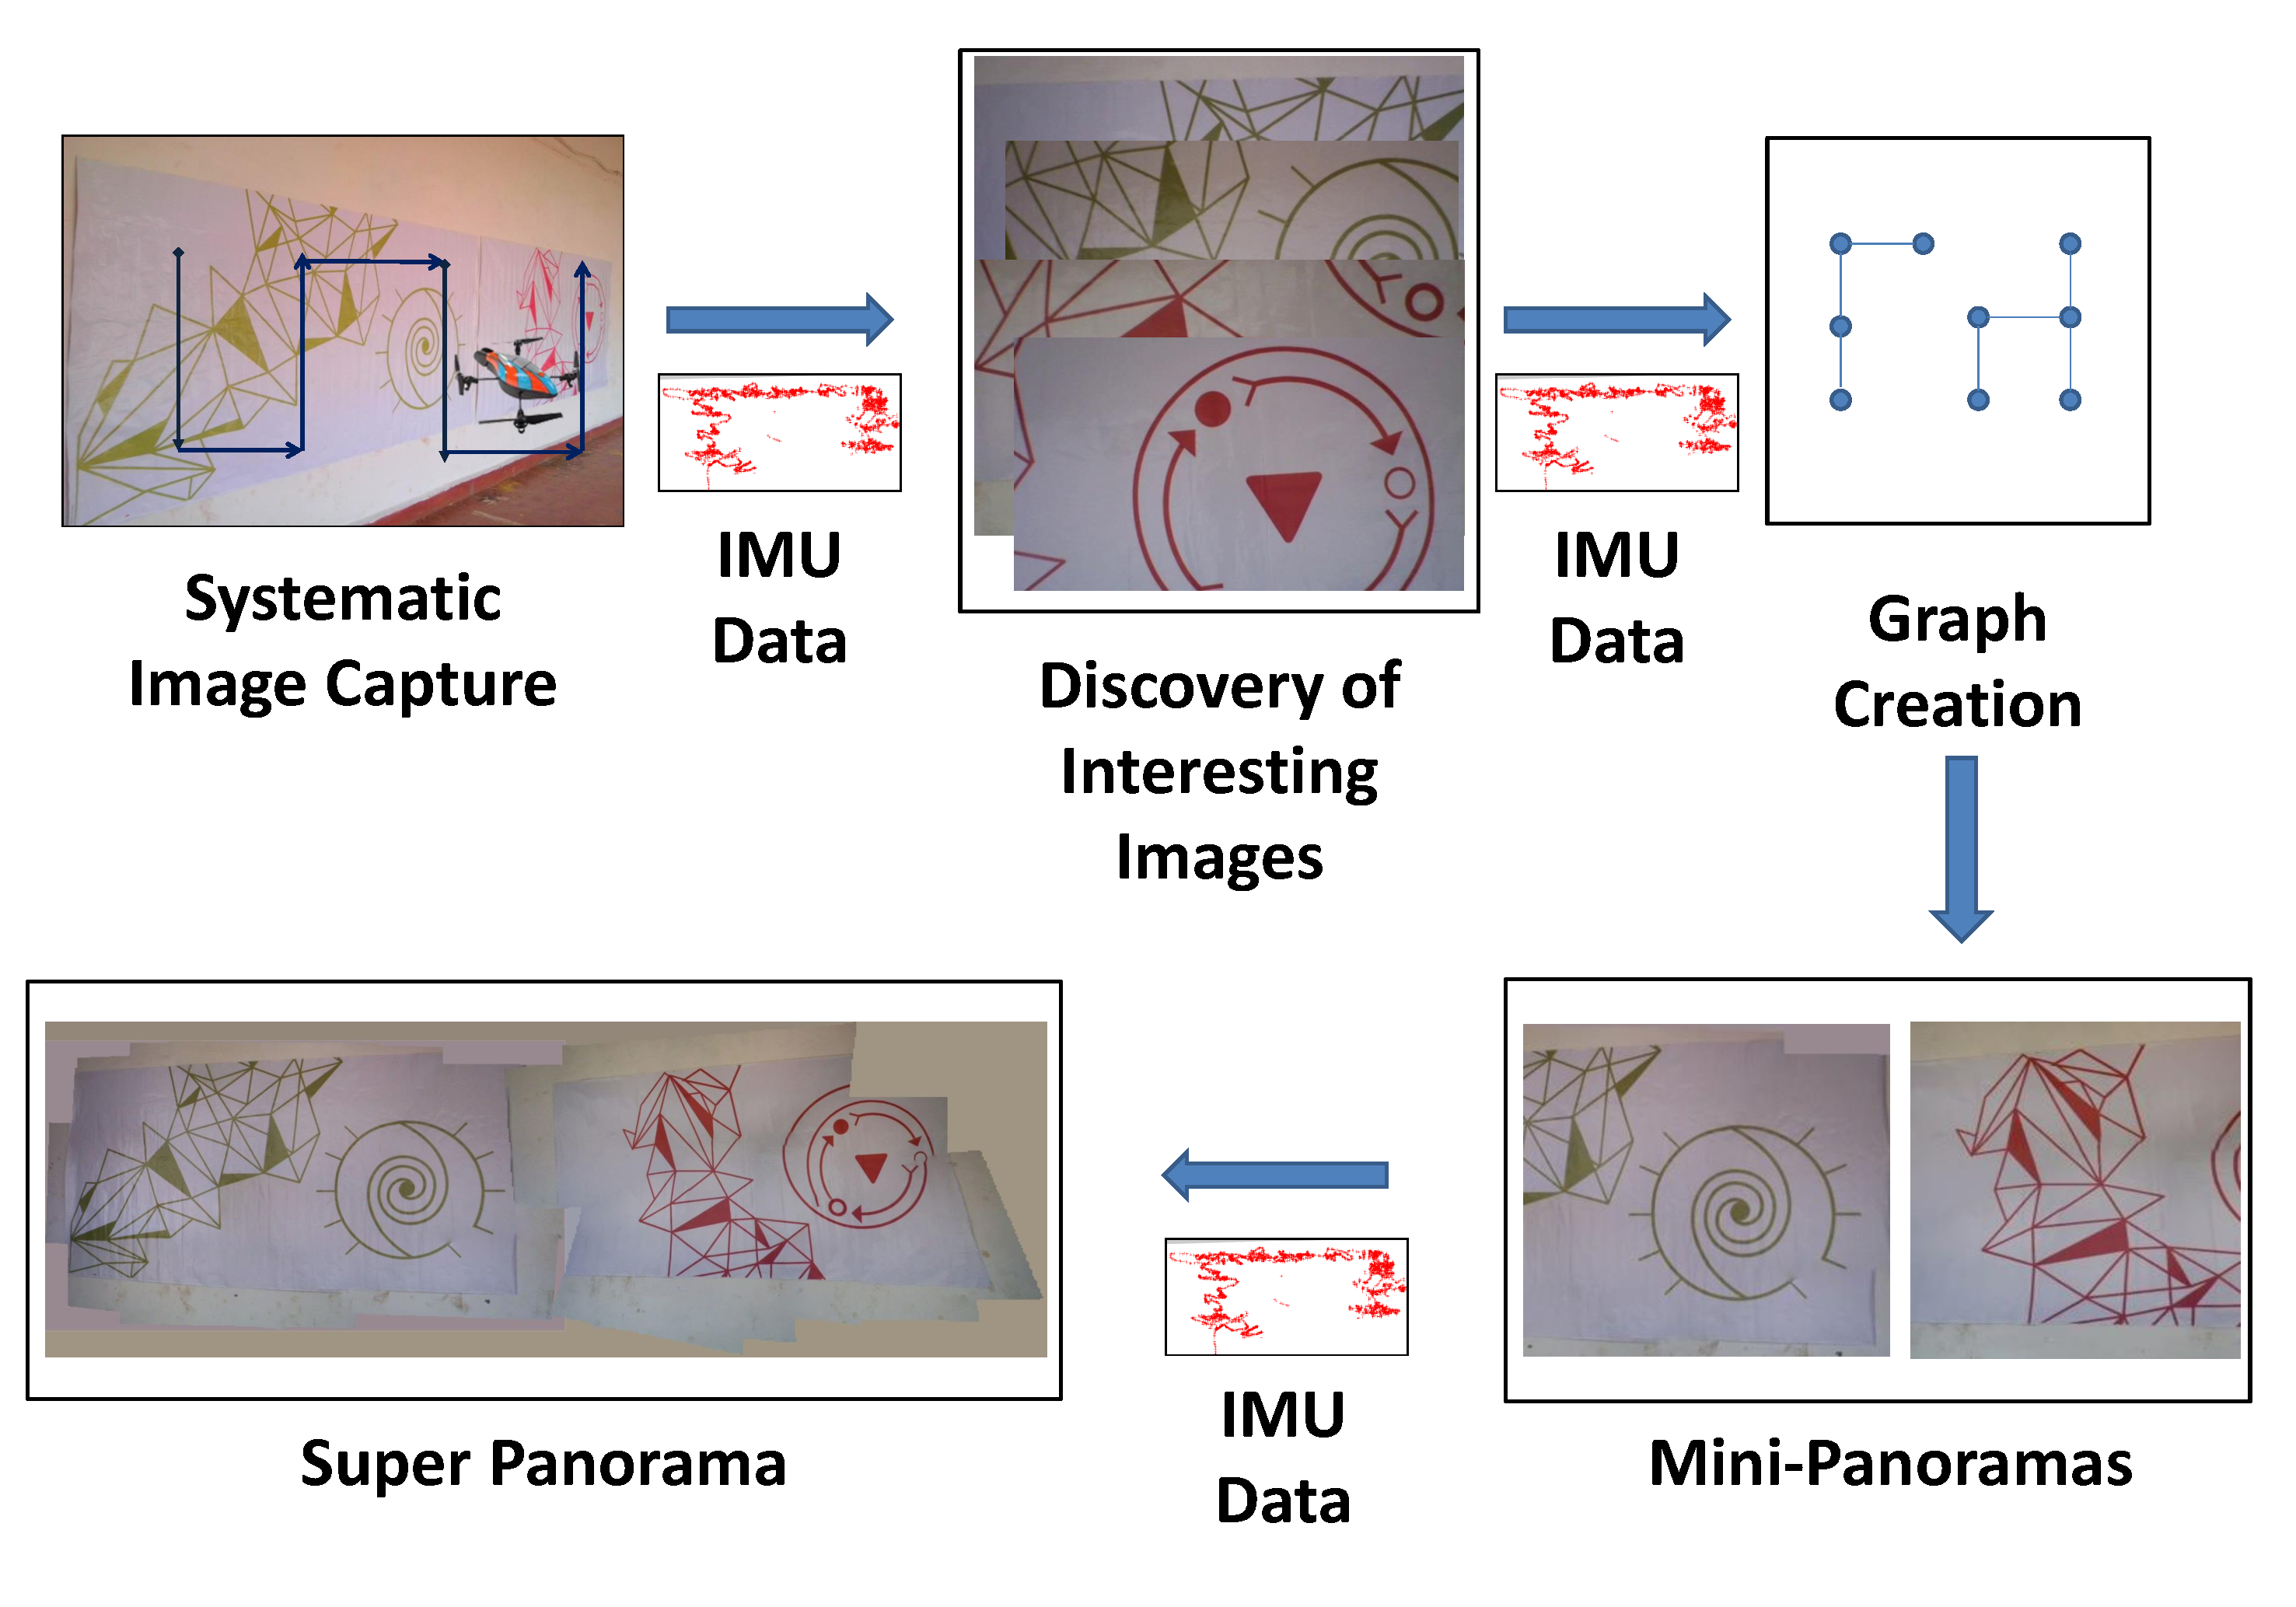
\includegraphics[width=\textwidth]{mosaicing/figures/Workflow} 
  \caption{ \label{fig:workflow} Overview: Input imagery is
    systematically acquired (top left) by a quadcopter.  In the next
    step, interesting images are found by clustering the video into
    regions based on positional data.  A graph is constructed using
    proximal images. For each connected component in a graph, standard
    stitching techniques are used to create mini-panoramas which are
    then joined together into super panorama 
    again using IMU data.}
\end{figure}
\subsection{Path Planning}
\subsection{Multi-planar Cases}

\section{Quadcopter-based Stagnant Water Identification}

Dengue~\cite{WHO15Dengue} is a troublesome debilating disease with no
known preventing vaccine, or cure. Doctors advocate that the best way
to avoid this disease is to avoid being bitten by mosquitoes which is
virtually an impossibility for many people in India.  The greatest
risk of contracting dengue (pronounced DENgee) is in the Indian
subcontinent.  

Technology is a must in tackling this situation.  The risk of disease
can be reduced by using insect repellents. In our institute, the
common method has been the spraying of insecticides.  Reports in the
media~\cite{china} indicate that China has flooded a small island
releasing half a million sterile mosquitoes to dominate the potent
mosquitoes. Such measures have unknown and unforeseen environmental
impact on the eco-system. Regardless, researchers are convinced that
there is no one single magic bullet to tackle the disease. 

Our work, started prior to the announcement of ``Project
Premonition,'' is similar to that of \cite{Microsoft15}.  Instead of
attempting to destroy the mosquito, we seek to detect the reason for
the increased outbreak, especially in urban areas.  The work reported
in this paper complements that of \cite{Microsoft15} --- the goal in \cite{Microsoft15}
is to ``catch wild mosquitoes'' (typically in the outfield) by
creating novel mosquito traps, and then to test mosquitoes for
pathogens. New traps are placed by drones, and retrieved by drones.
In contrast, this paper emphasizes the need for identifying the
location of these traps.  

One of the major reasons behind the growth of mosquitoes is the
continuous existence of \emph{water puddles} around residencies in
urban India.  The virus is carried by mosquitoes, and these breed in
stagnant water. \emph{Can we detect stagnant water?}  When we surveyed
terraces (Fig.~\ref{teaser}) and ``chajjas'' of various buildings in
our institute, we found split AC air conditioners dumping condensed
water. Such areas can be surveyed using autonomous quadcopters.

\subsection{Related Work}
The method in ~\cite{santana12} for detection of
water relies on the chaotic nature of water's dynamic texture to
exploit a measure of entropy over the trajectories obtained from
optical flow trackers over several frames. \cite{zhang10} has
introduced a descriptor which is tolerant to the flip transformation
and even non-rigid distortions, such as ripple effects.  \emph{These
  methods and others in the literature focus on the turbulent aspects
  of water}, largely absent in our application that focuses on
stagnant water.  Our method is closest to that of Rankin et
al.~\cite{rankin2004daytime, rankin11} who have implemented a rule-based water
detector based on sky reflections.  These rules are established
based on an analysis of images captured in wide-open areas on
cross-country terrain. Not only do we have new methods, \emph{our
datasets are captured in urban areas using a quadcopter and thus these
rules seem unlikely to be readily applicable.}

\subsection{Methodology}
Our method is based on a combination of color based method with an optical flow
based method.  We establish the need for the combination in the first two subsections.

\noindent\textbf{Appearance-based Detection}

\begin{figure}[h!]
  \centering
  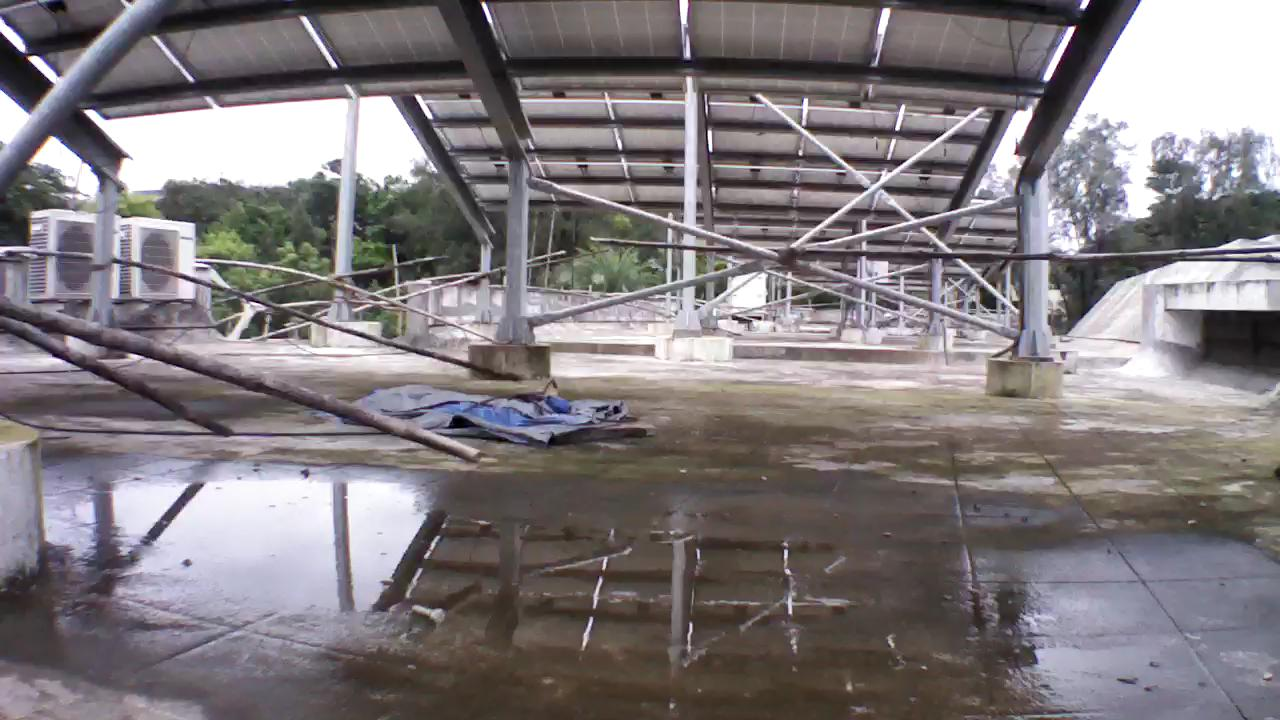
\includegraphics[width=0.4\linewidth]{stagnantWater/figures/IMG_PAIR_27_1}
  \hfill
  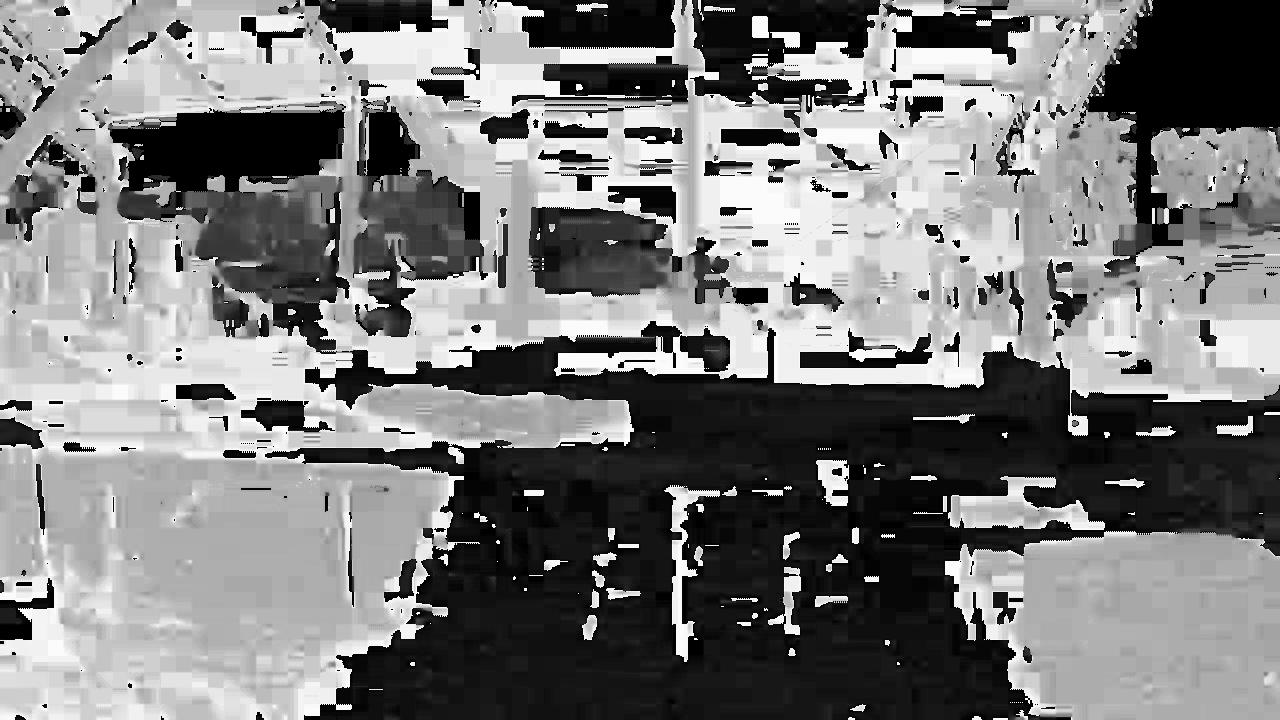
\includegraphics[width=0.4\linewidth]{stagnantWater/figures/IMG_PAIR_27_1_H} 

  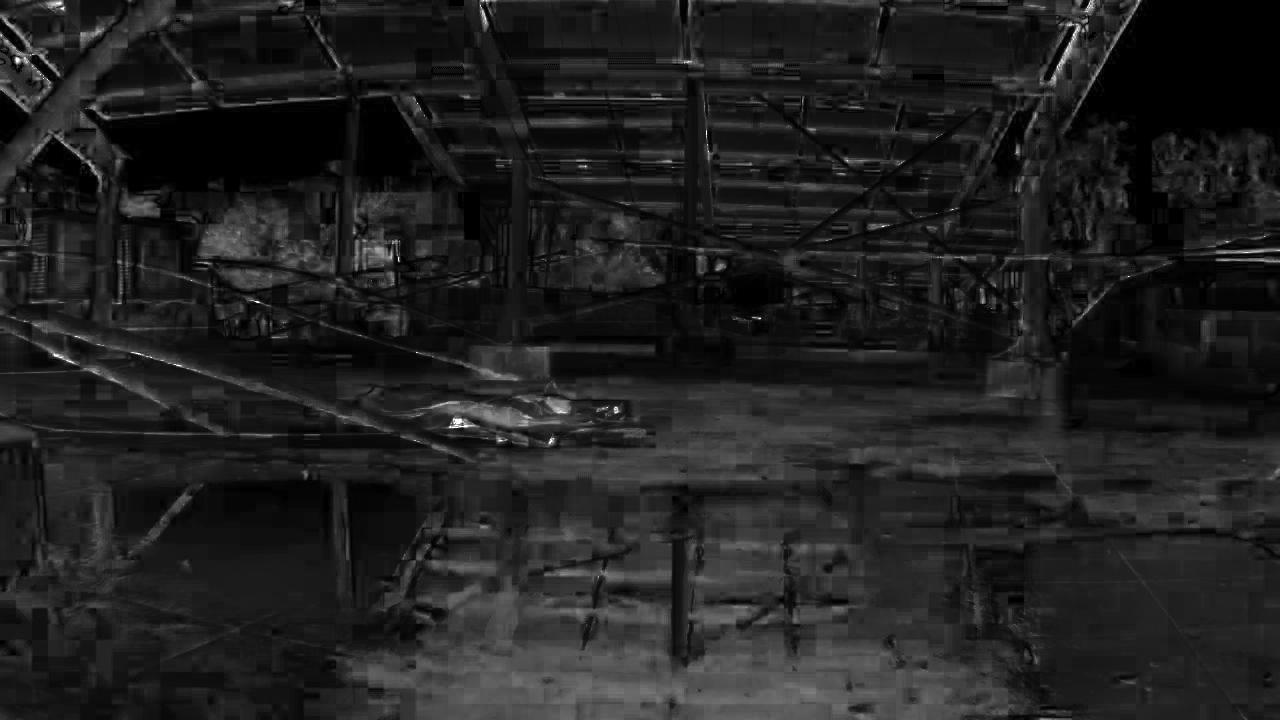
\includegraphics[width=0.4\linewidth]{stagnantWater/figures/IMG_PAIR_27_1_S}
  \hfill
  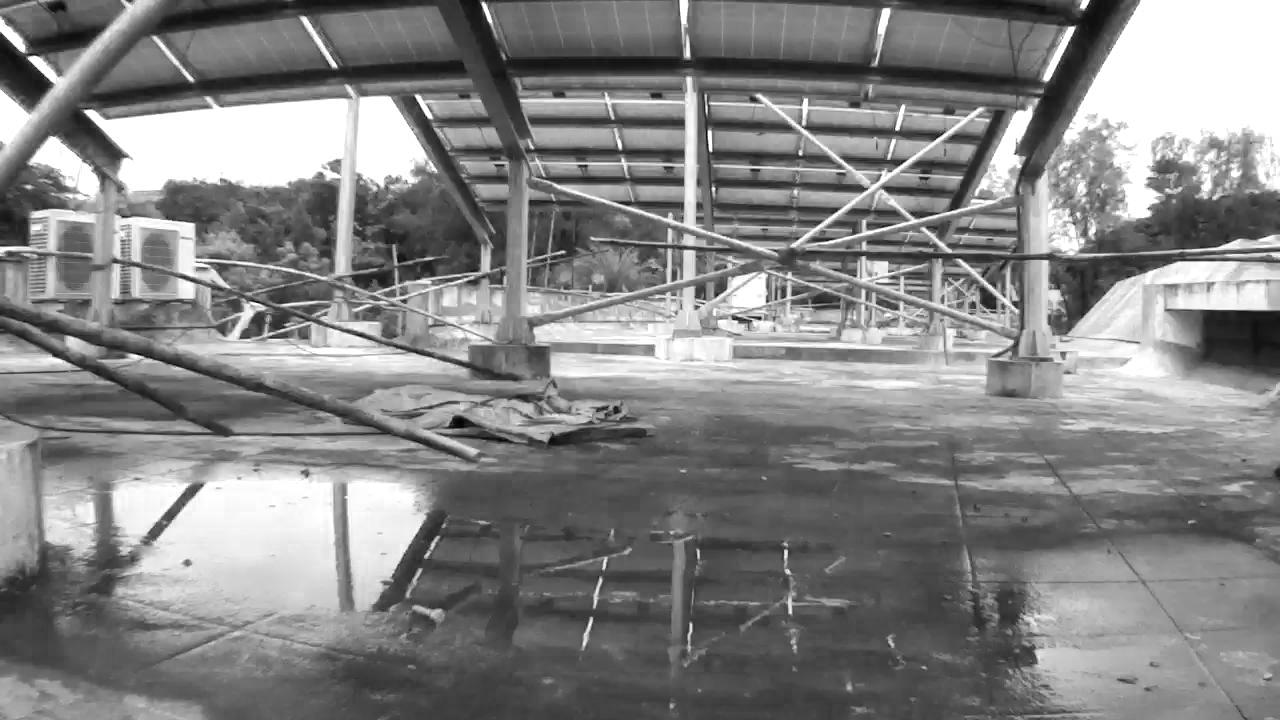
\includegraphics[width=0.4\linewidth]{stagnantWater/figures/IMG_PAIR_27_1_V}
  \caption{An image (top left) and the HSV components.  The puddle has
    low saturation (bottom left) but high intensity (bottom right).
    The hue is indeterminable and is based on the environment.}
  \label{fig:HSV}
\end{figure}

Under ambient lighting conditions, puddle areas display high
brightness and low saturation as can be seen in
Fig.~\ref{fig:HSV}. Features based on these are fed to an SVM
classifier. Training an SVM is a labour intensive task.  To reduce the
effort, we have developed a tool shown in Fig.~\ref{fig:training}. 

\begin{figure}[h!]
  \centering
  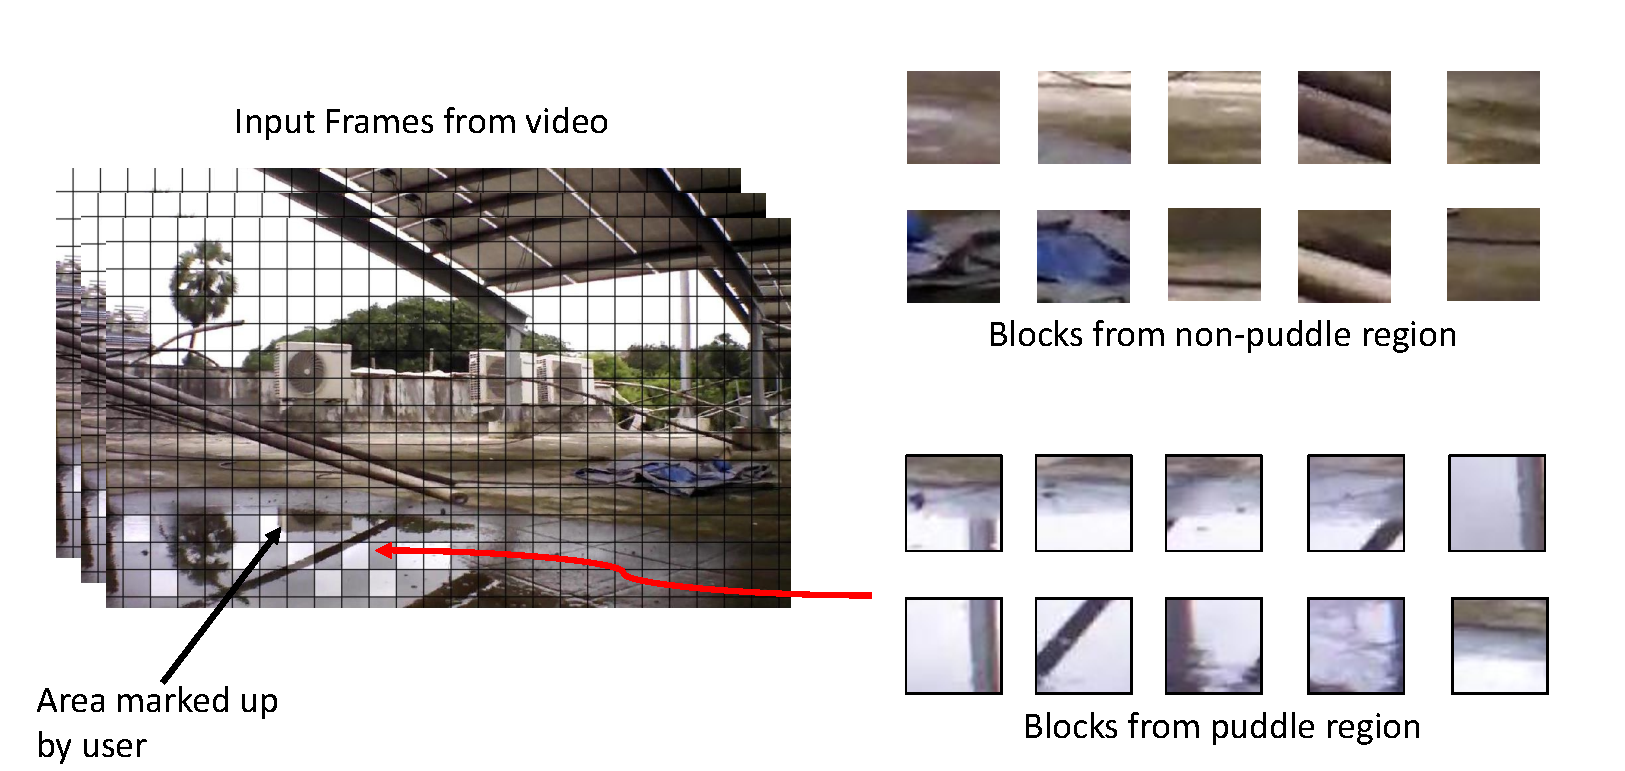
\includegraphics[width=0.9\linewidth]{stagnantWater/figures/trainingData.pdf}
  \caption{The process for creation of training data. The user selects
    the stagnant water area by drawing a contour to produce `positive'
    and `negative'  data.}
  \label{fig:training}
\end{figure}

\textbf{Failure of SVM-based methods:} The SVM detector is good at
detecting regions of sky reflected off a puddle.  In the HSV color
space, these regions have low saturation (S) and high brightness (V)
values, and are picked up with high reliability by the HSV histogram
feature based SVM detector. However, false negatives are also produced
since other reflected regions such as trees, buildings, etc. are
usually classified as non-puddle regions as many of these
characteristics is shared by negative images in the training data set.
\vspace{0.5cm}

\noindent\textbf{Optical flow based Detection}
Fortunately our images are captured by a moving quadcopter.  The
optical flow measures apparent motion of objects in a scene caused by
relative motion between camera and object. The magnitude of the
optical flow is high for objects that are close in comparison to
objects at a distance.  Fig.~\ref{fig:optical_flow} shows the
magnitude of optical flow calculated from two images.

\begin{figure}[h!]
  \centering
  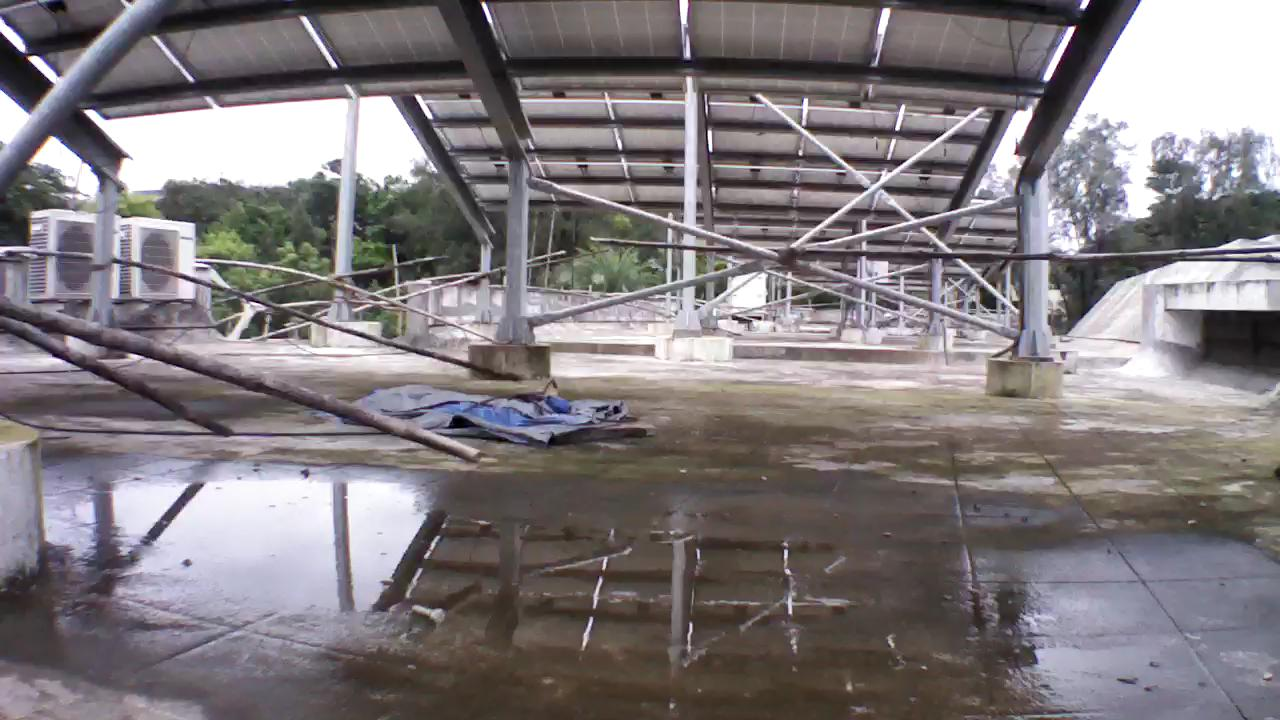
\includegraphics[width=0.32\linewidth]{stagnantWater/figures/IMG_PAIR_27_1}
  \hfill
  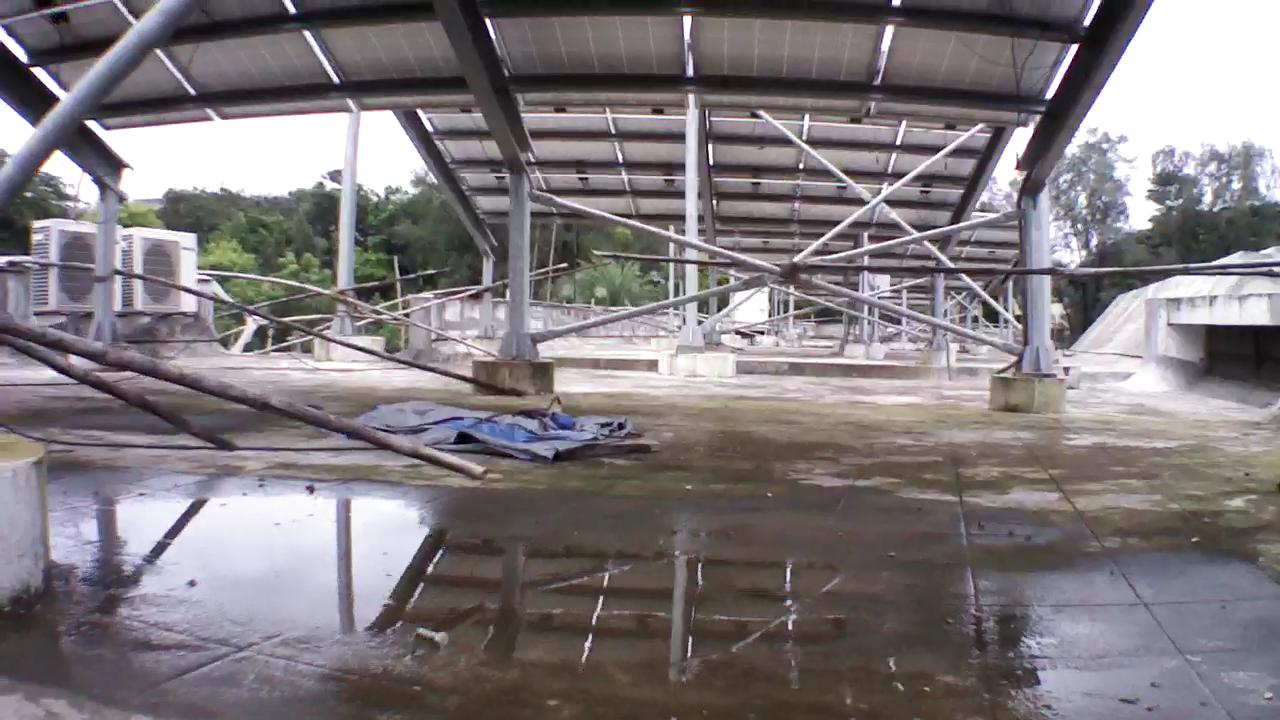
\includegraphics[width=0.32\linewidth]{stagnantWater/figures/IMG_PAIR_27_2}
  \hfill
  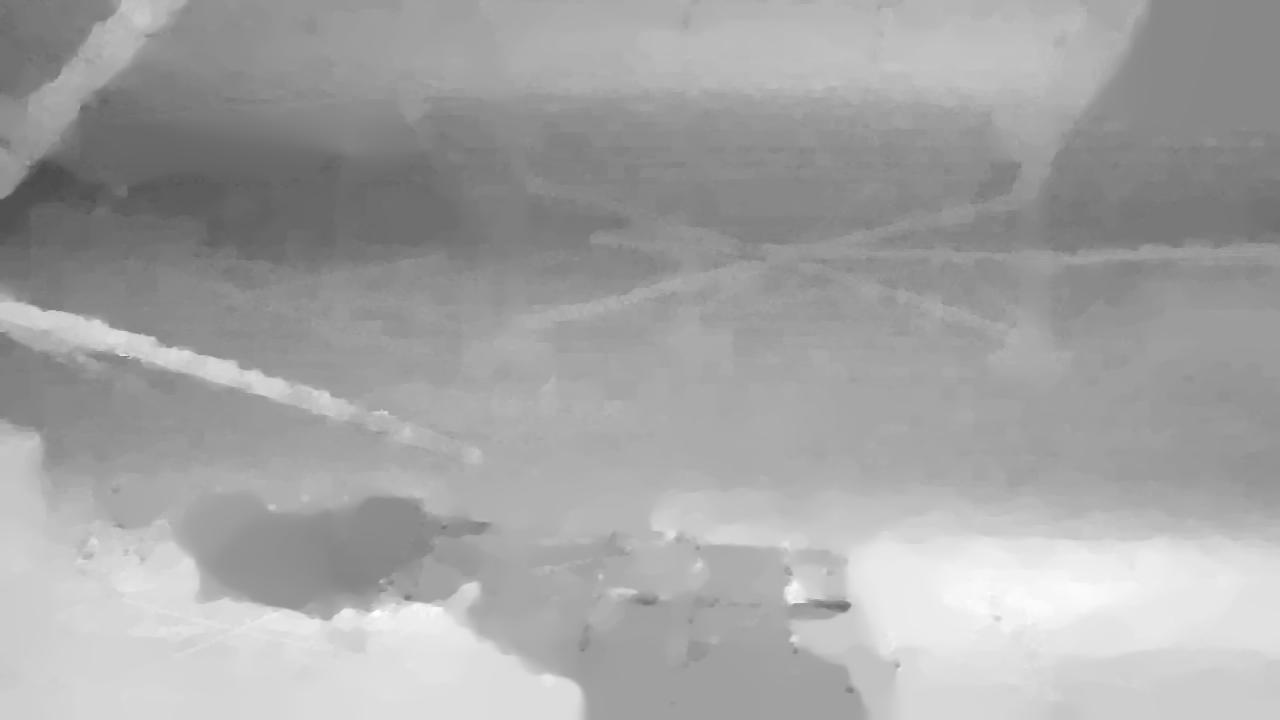
\includegraphics[width=0.32\linewidth]{stagnantWater/figures/IMG_PAIR_27_optical_flow}
  \caption{Optical Flow. Left, Middle: Frames taken from positions
    which are $d$ units apart in 3D world. $ 0.01 \leq d \leq 0.1$. Right:
    Magnitude of optical flow. We observe that the magnitude of optical
    flow in the reflective parts of the puddle is relatively low.}
  \label{fig:optical_flow}
\end{figure}

A recent thesis \cite{Liu11Thesis} has one of the state of the art
algorithm for optical flow. One requirement is the need for
spatio-temporal smoothness constraint which can be challenging because
of the jerky movement of the UAV.  To resolve this, we use the
Inertial Measurement Unit (IMU) data available on the quadcopter to
synchronize positional information with the video sequence captured by
quadcopter. In short, we select the frame pair which are spatially the
closest, among a set of competing temporally adjacent frames.

\textbf{Failure of optical flow:} Optical flow is essentially being
used in a depth from parallax mode to exploit the fact that still
puddles behave like mirrors. The scenery reflected by such puddles is
usually at a much greater depth than the immediate surroundings of the
puddle.  Optical flow is largely independent of hue and saturation.
For the same reason, however, optical flow as a means of detecting
puddles will fail to report true positives when the object that is
being reflected is close by. In such cases, the saturation and
intensity values are useful.

Yet another reason for the failure for the optical flow is the
inability to distinguish true ``far away'' regions versus imagined far
away regions due to the mirror-like properties of water.  To handle
these false positives, we devise a horizon mask based on the principle
that water flows down.

\textbf{Combined approach}

\textbf{Horizon Mask:} The change in depth for far-away scenes as well
as their ref	lections on puddle, in consecutive frames, are hard to
distinguish. In previous work \cite{rankin11} such issues are avoided
by discarding a fixed-portion of image corresponding to far-off
regions, enforced by constrained input capture method. Due to
inapplicability of such constraints in the comparatively agile input
capture conditions of quadcopter, features derived from urban
environment are utilized for finding plausible puddle regions. In
urban setting, the high availability of structures in surroundings,
having distinctly flat surfaces and rectilinear silhouettes, enables
use of edge-detection based methods to bound planar regions that can
contain puddle. Applying the Hough transform with calibrated
parameters followed by length-based selection of lines detected, a
upper boundary for puddle region called `Horizon' is found. The
Horizon is in turn used to create a binary mask to be applied to local
scores from other techniques before normalization.

\begin{figure}[h!]
  \centering
  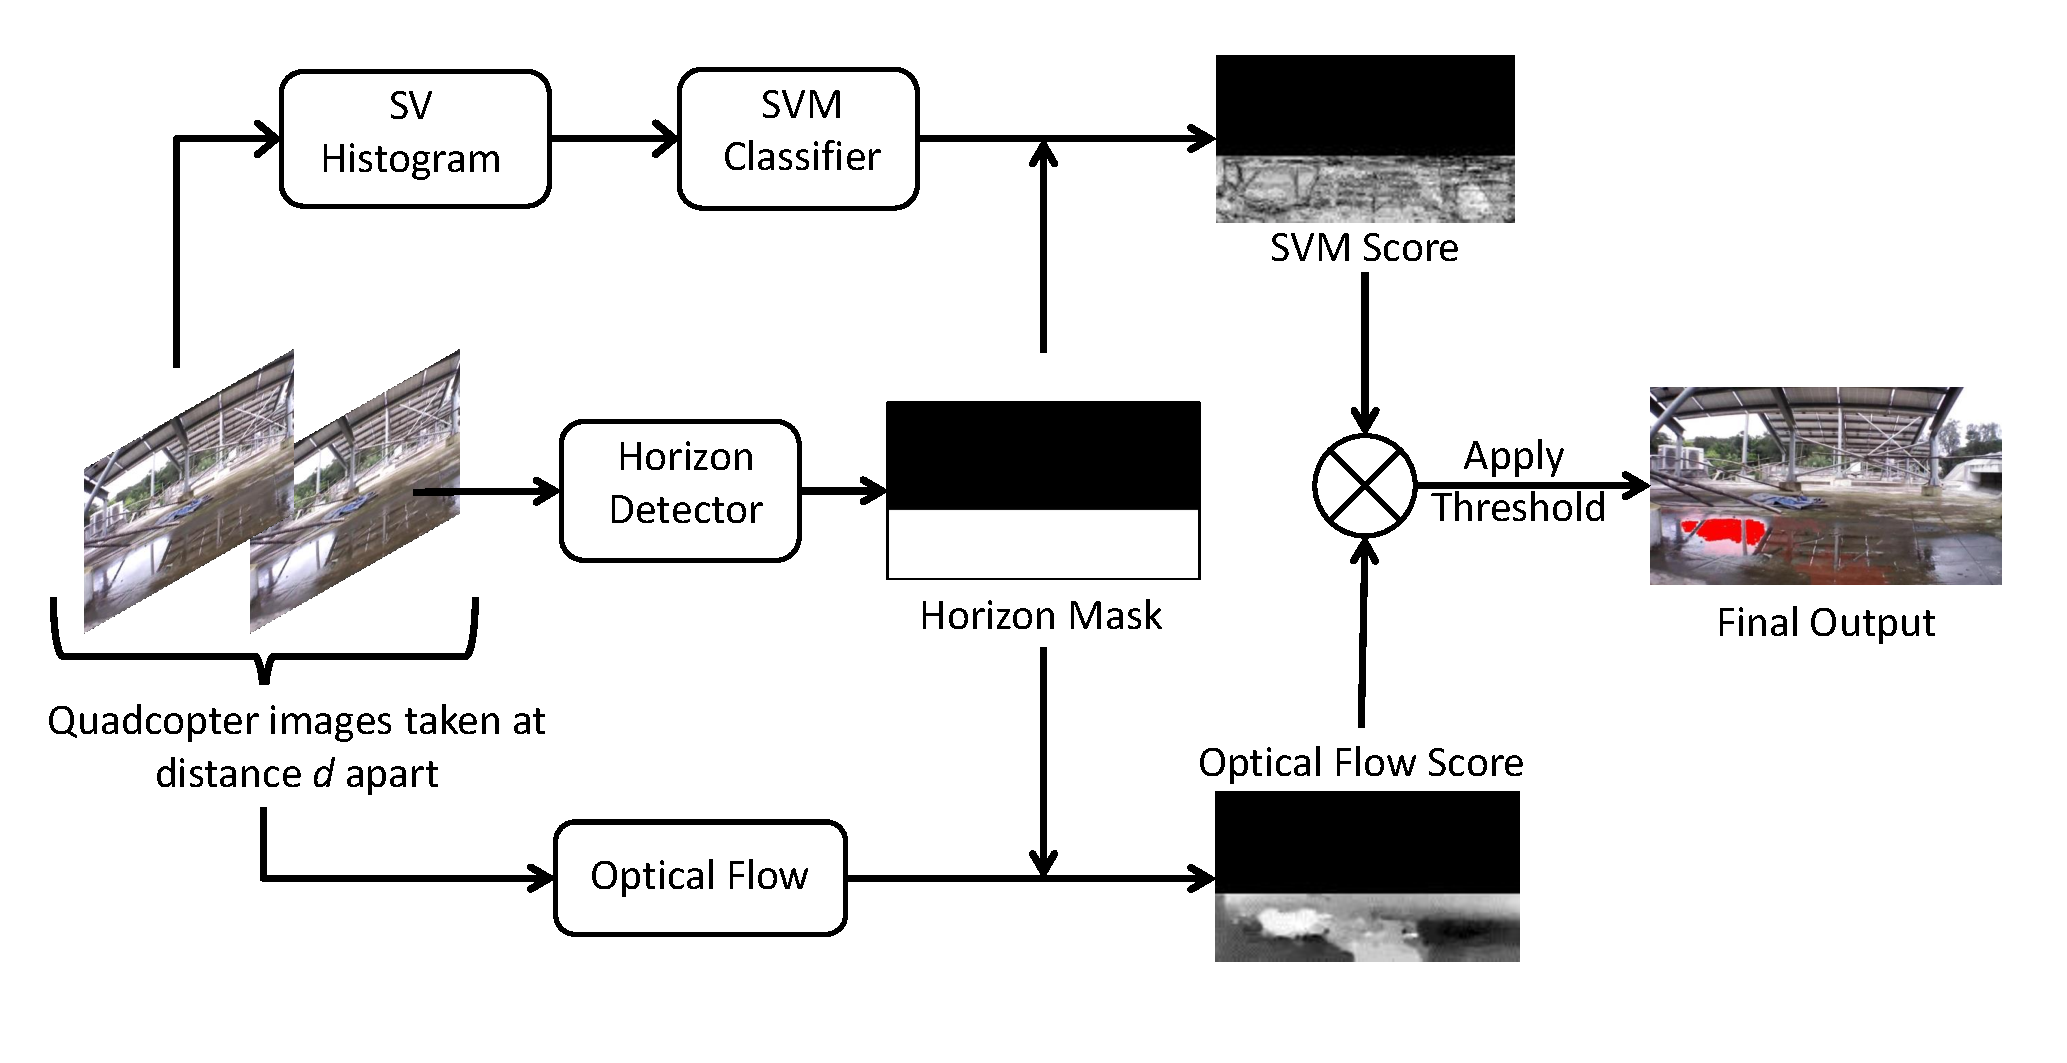
\includegraphics[width=\textwidth]{stagnantWater/figures/overall_workflow.pdf}
  \caption{Overall architecture.}
  \label{fig:workflow}
\end{figure}

These observations suggested a novel combined approach as sketched
in Fig.~\ref{fig:workflow}.

\subsection{Experiments and Results}

All our experiments have been completed with the inexpensive consumer
quadcopter called Parrot's AR Drone. We remark that one should not
compare expensive military grade drones with such inexpensive drones.
For the purpose of showing the efficacy of this paper, we also took a
picture of the scene from a distance with a 5 mega-pixel camera for
the reader to better understand the scene.  We covered urban places
such as terraces, constructions sites, building backyards,
pumping stations, and so on.  We have captured around eight different
types of datasets, each having around two-three minutes of video
(around 3000 frames each). 

\textbf{Comparison:} We compare our method to \cite{rankin2004daytime} on
representative images since the methods in \cite{rankin11} do not apply. 
%See Fig.~\ref{fig:comparison}. 
It can be seen
from Fig.~\ref{fig:comparison} that in all images, \cite{rankin2004daytime} is
confusing  bright patches as puddle patches (note red patches on walls, sky etc.
in middle column in Fig.~\ref{fig:comparison}). Also, \cite{rankin2004daytime}
is not able to detect textured puddle images (as seen in the first row in
Fig.~\ref{fig:comparison}). (The confidence in detection is indicated by red
hue in the output image. So, darker the red tinge, higher the confidence in
detected water region. )

\begin{figure}
  \centering
   
  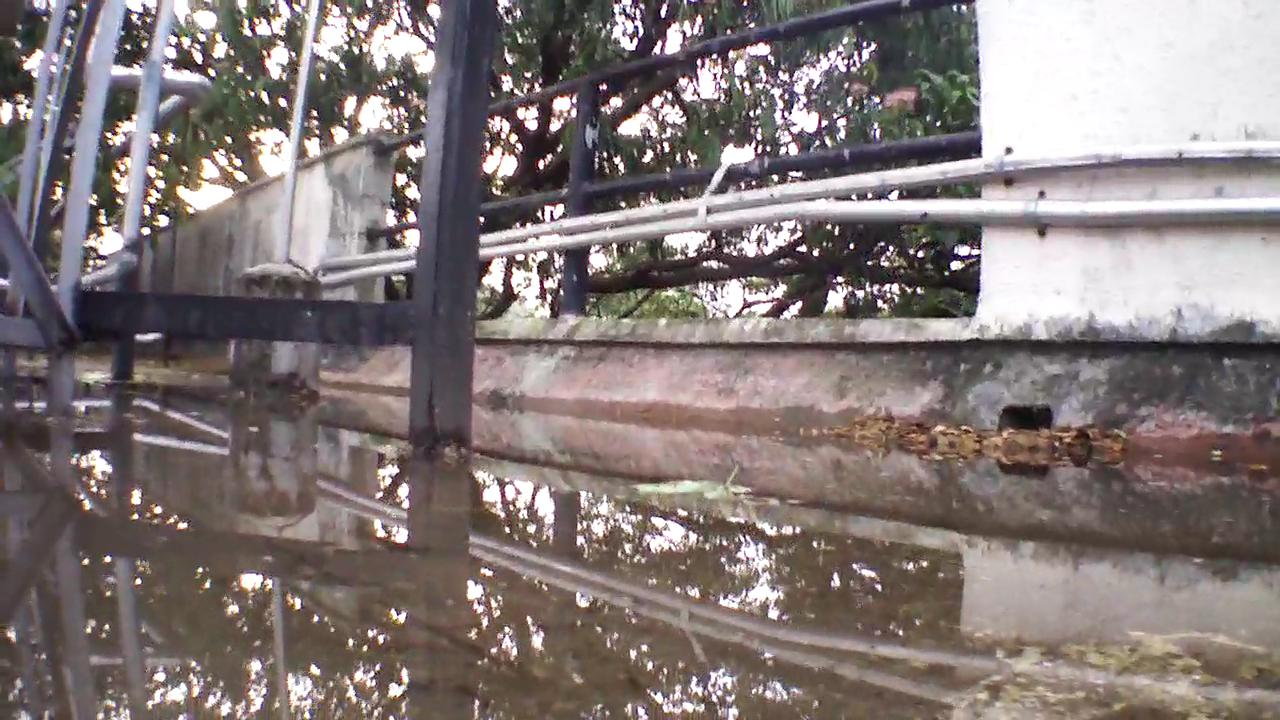
\includegraphics[width=0.32\linewidth]{stagnantWater/results/dataset_73/IMG_PAIR_124_1} \hfill
  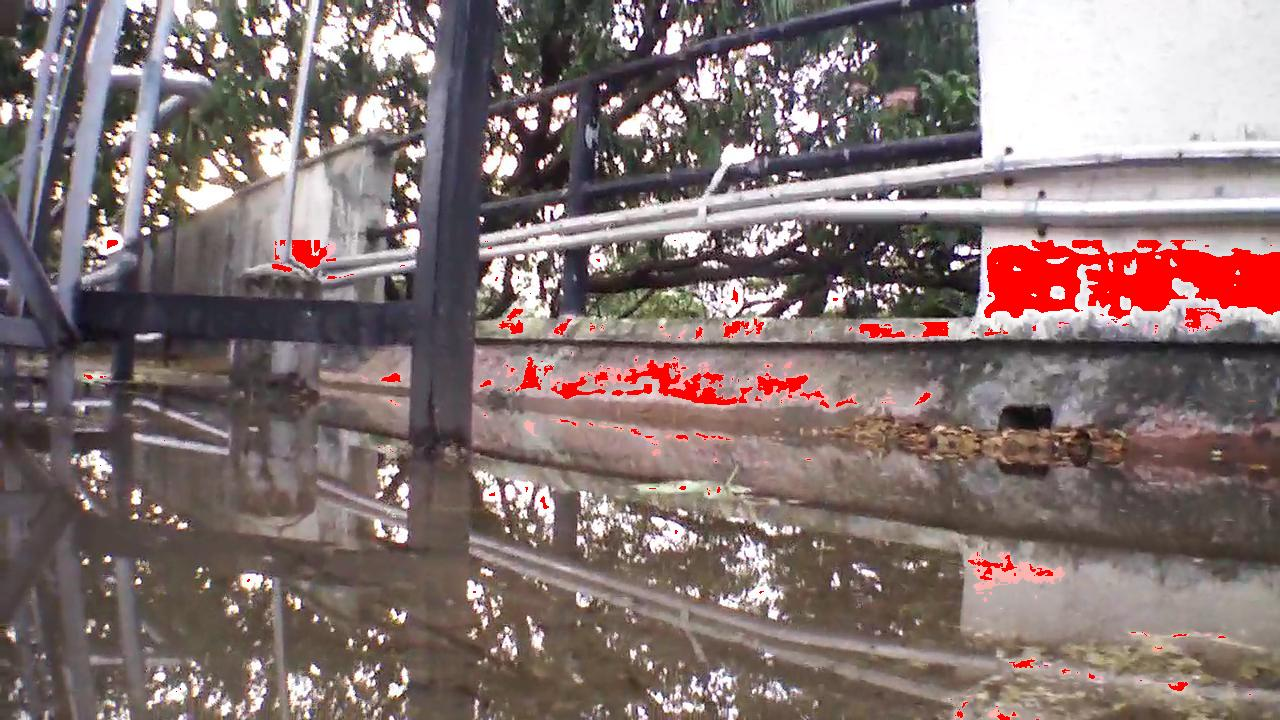
\includegraphics[width=0.32\linewidth]{stagnantWater/results/dataset_73/output_124_jpl2} \hfill
  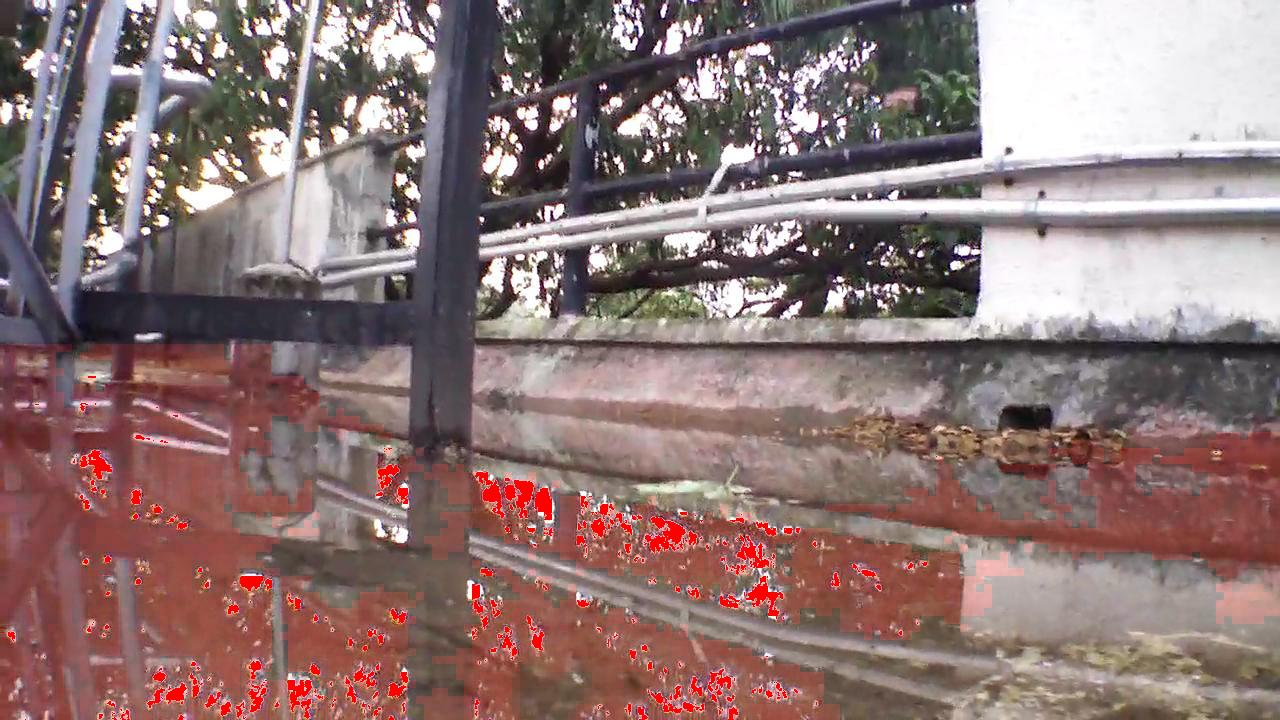
\includegraphics[width=0.32\linewidth]{stagnantWater/results/dataset_73/output_124}

  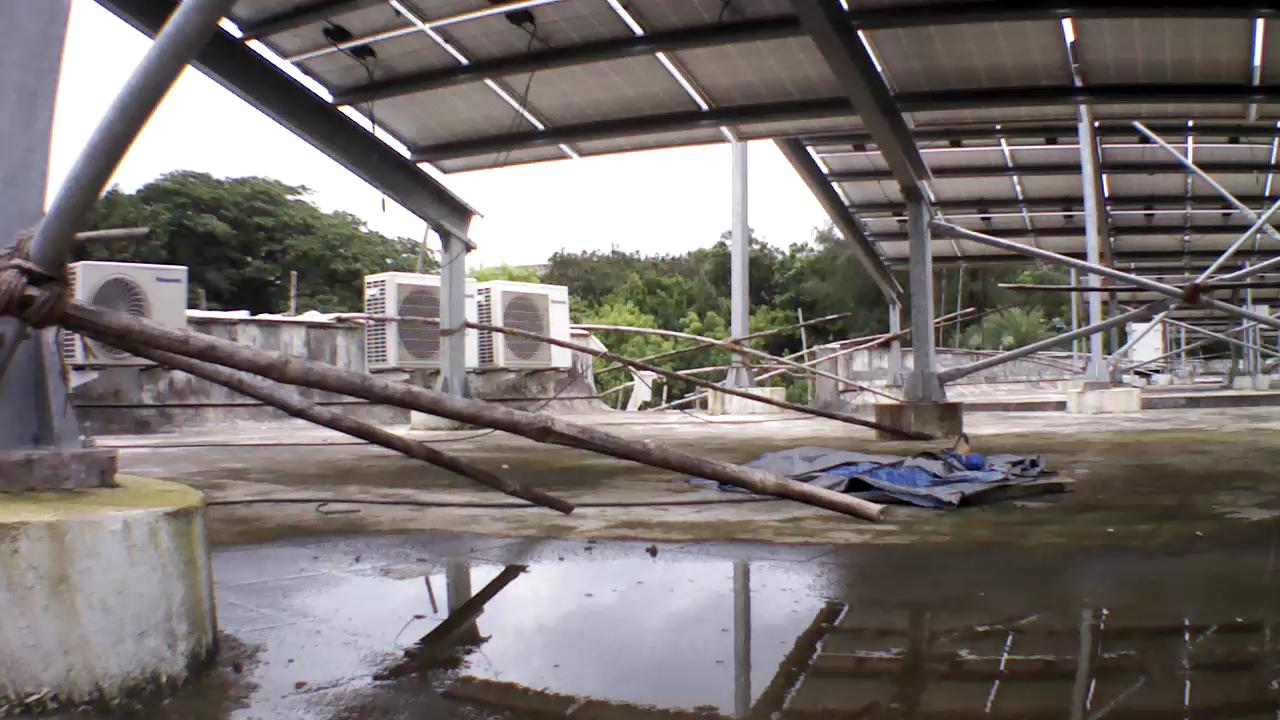
\includegraphics[width=0.32\linewidth]{stagnantWater/results/dataset_81/IMG_PAIR_1_1} \hfill
  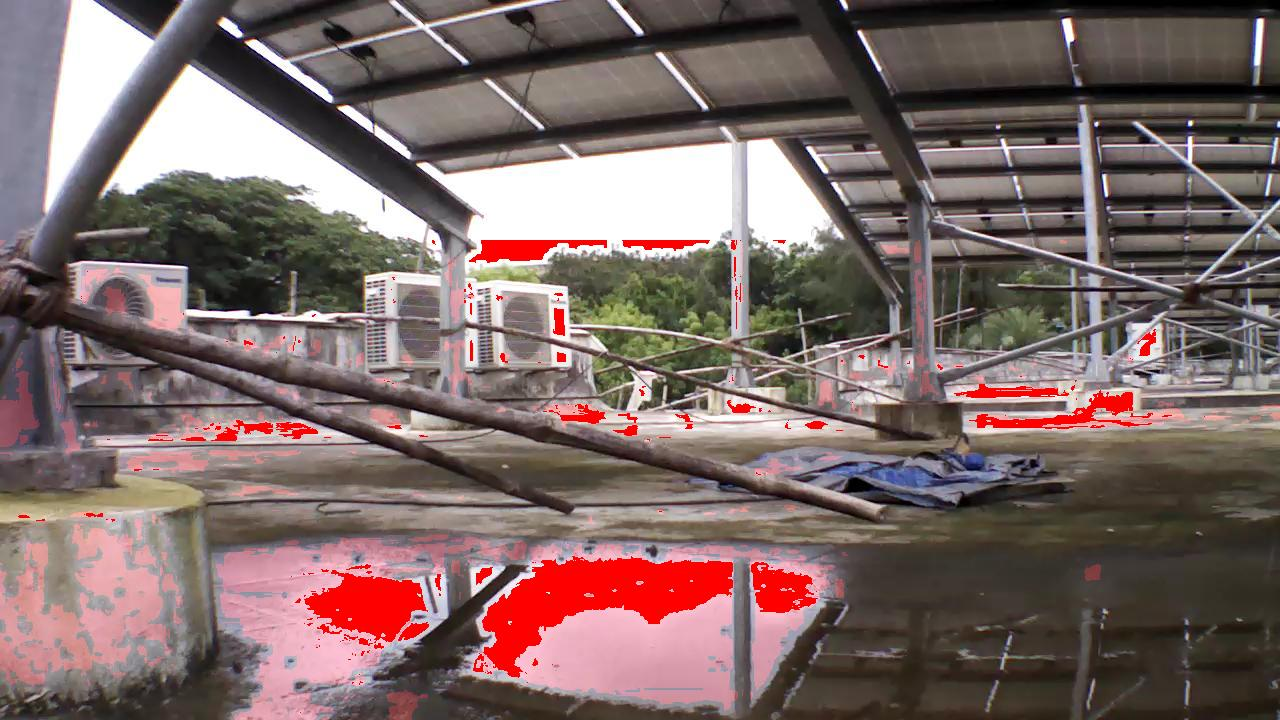
\includegraphics[width=0.32\linewidth]{stagnantWater/results/dataset_81/output_1_jpl2} \hfill
  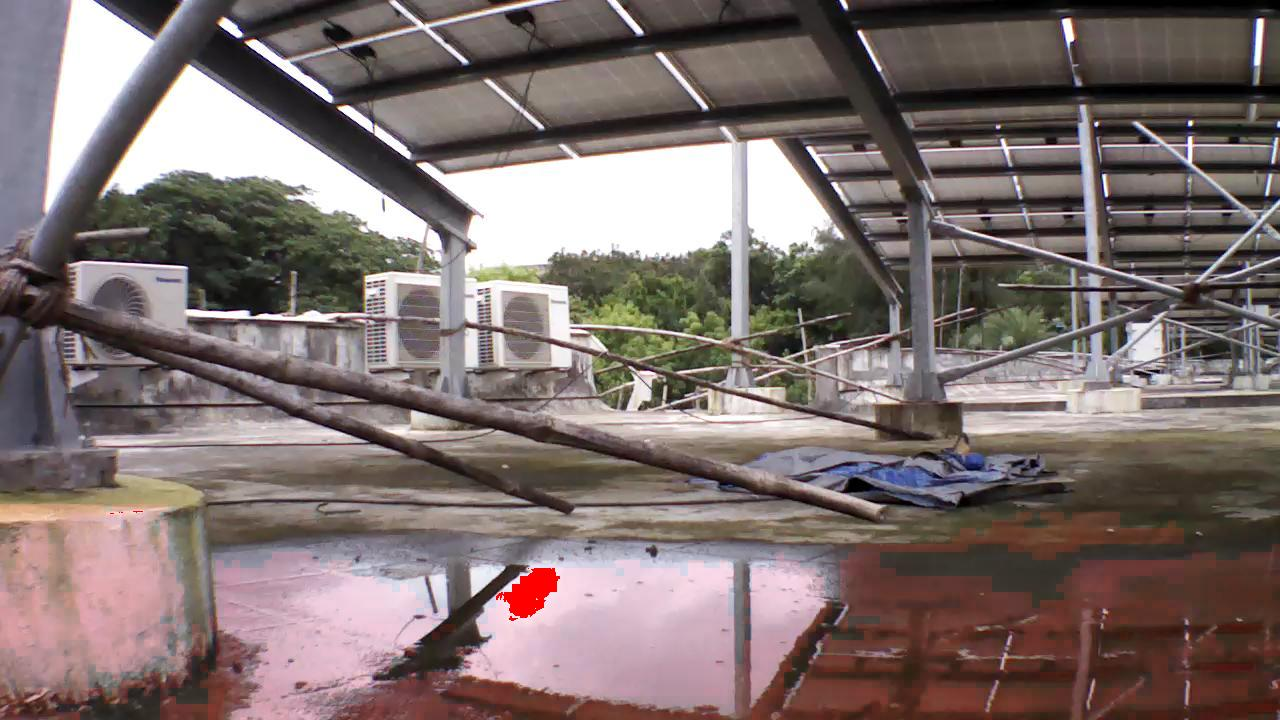
\includegraphics[width=0.32\linewidth]{stagnantWater/results/dataset_81/output_1}

  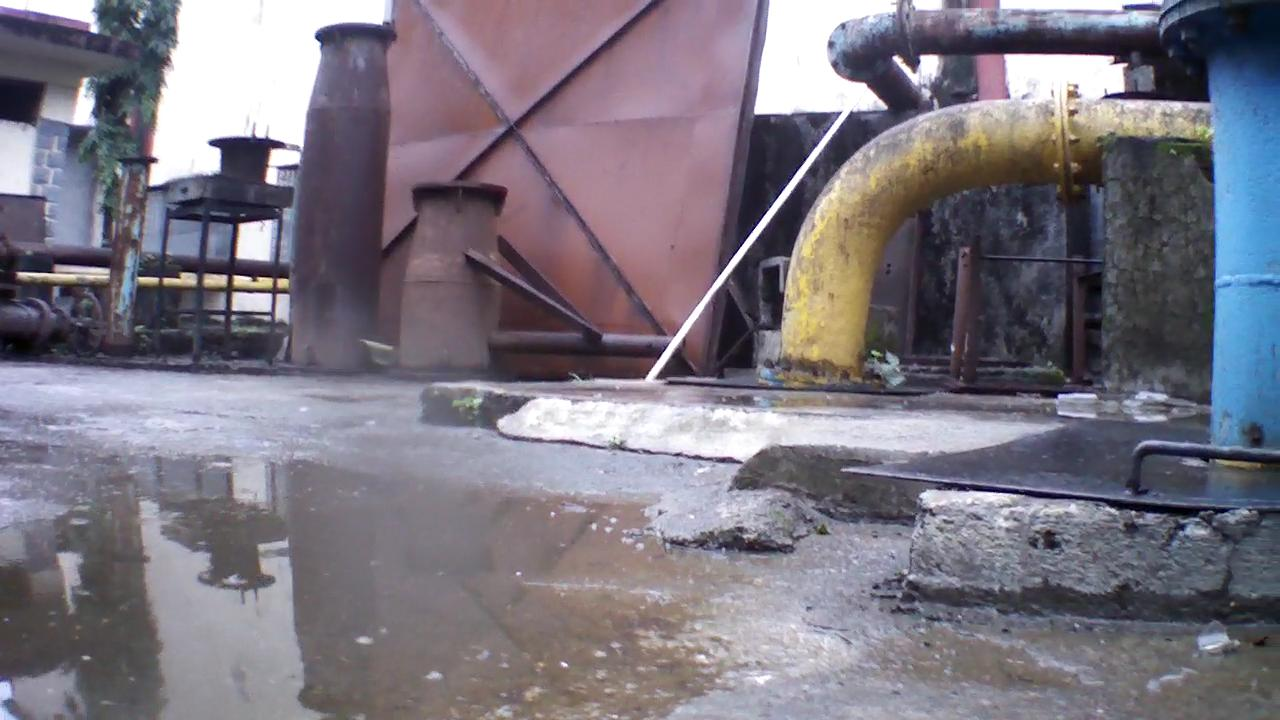
\includegraphics[width=0.32\linewidth]{stagnantWater/results/dataset_82/IMG_PAIR_192_1} \hfill
  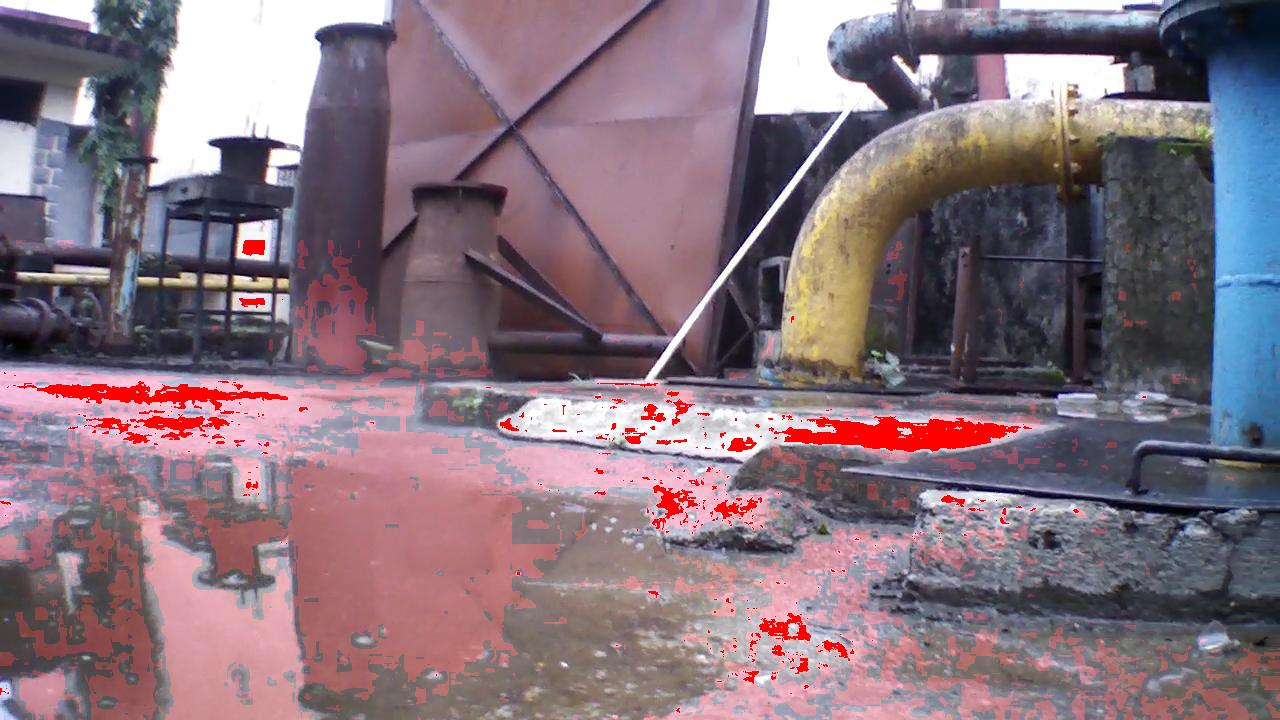
\includegraphics[width=0.32\linewidth]{stagnantWater/results/dataset_82/output_192_jpl2} \hfill
  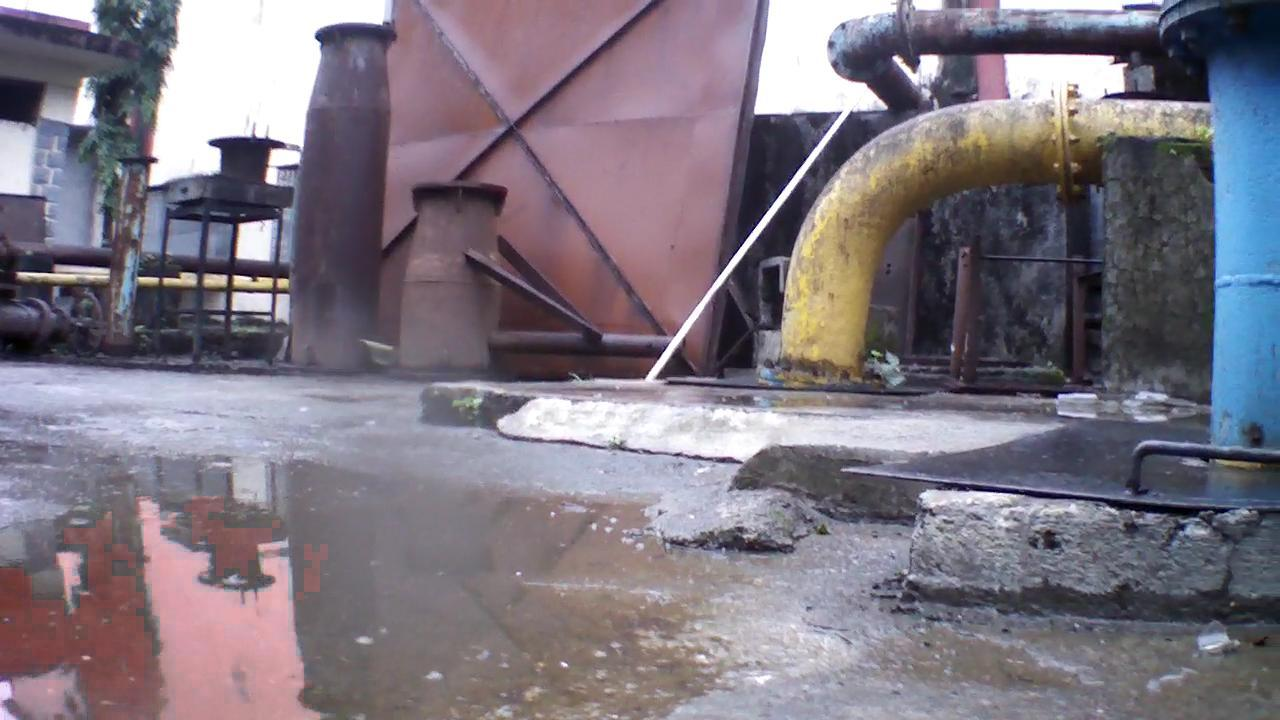
\includegraphics[width=0.32\linewidth]{stagnantWater/results/dataset_82/output_192}
  
  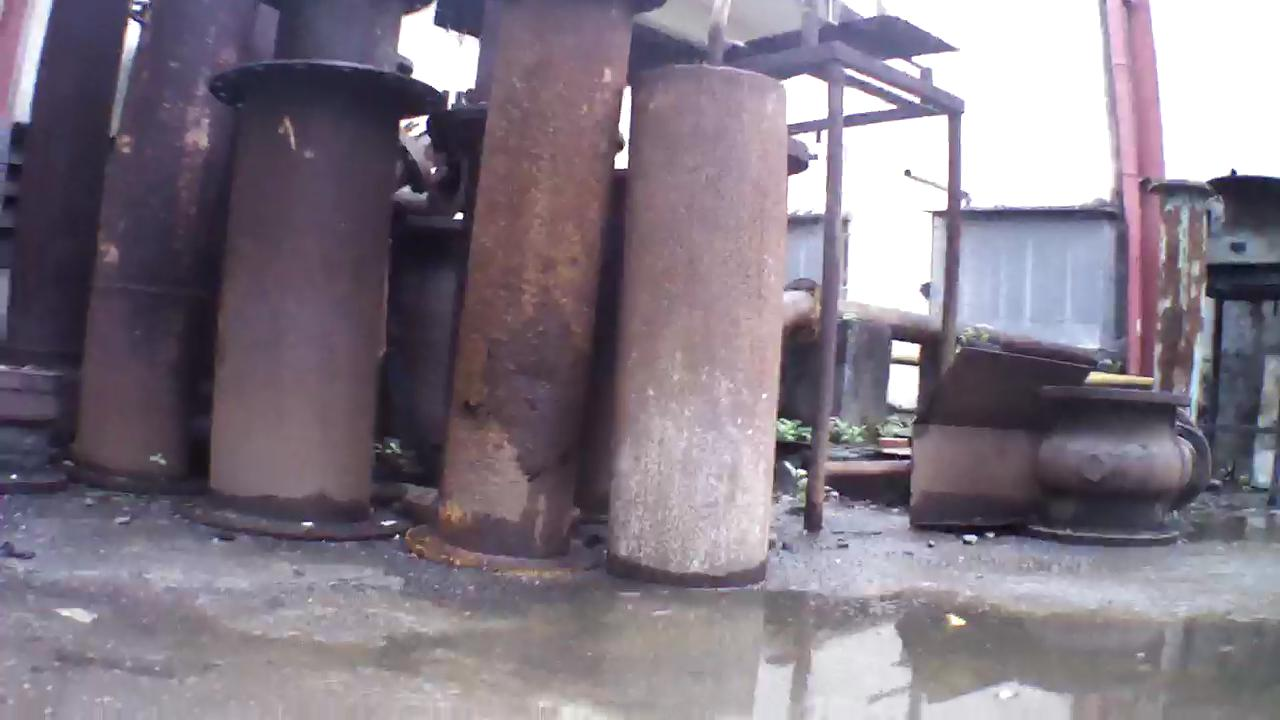
\includegraphics[width=0.32\linewidth]{stagnantWater/results/dataset_83/IMG_PAIR_130_1} \hfill
  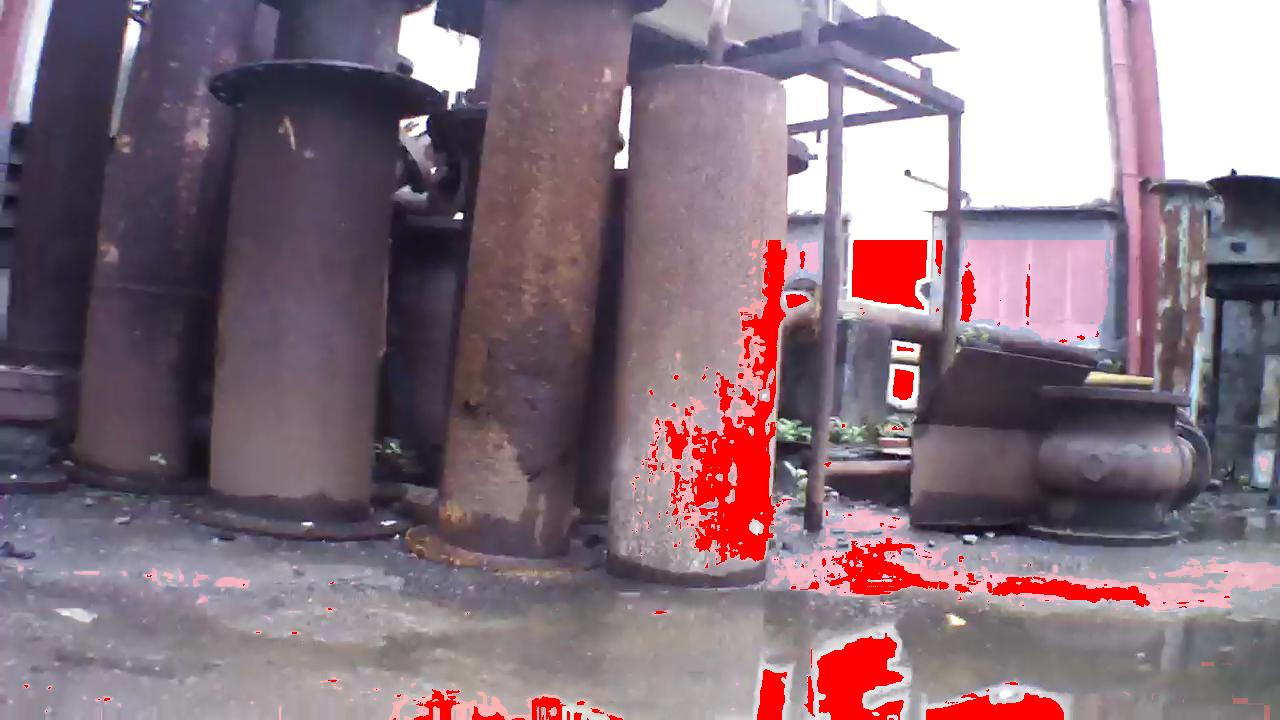
\includegraphics[width=0.32\linewidth]{stagnantWater/results/dataset_83/output_130_jpl2} \hfill
  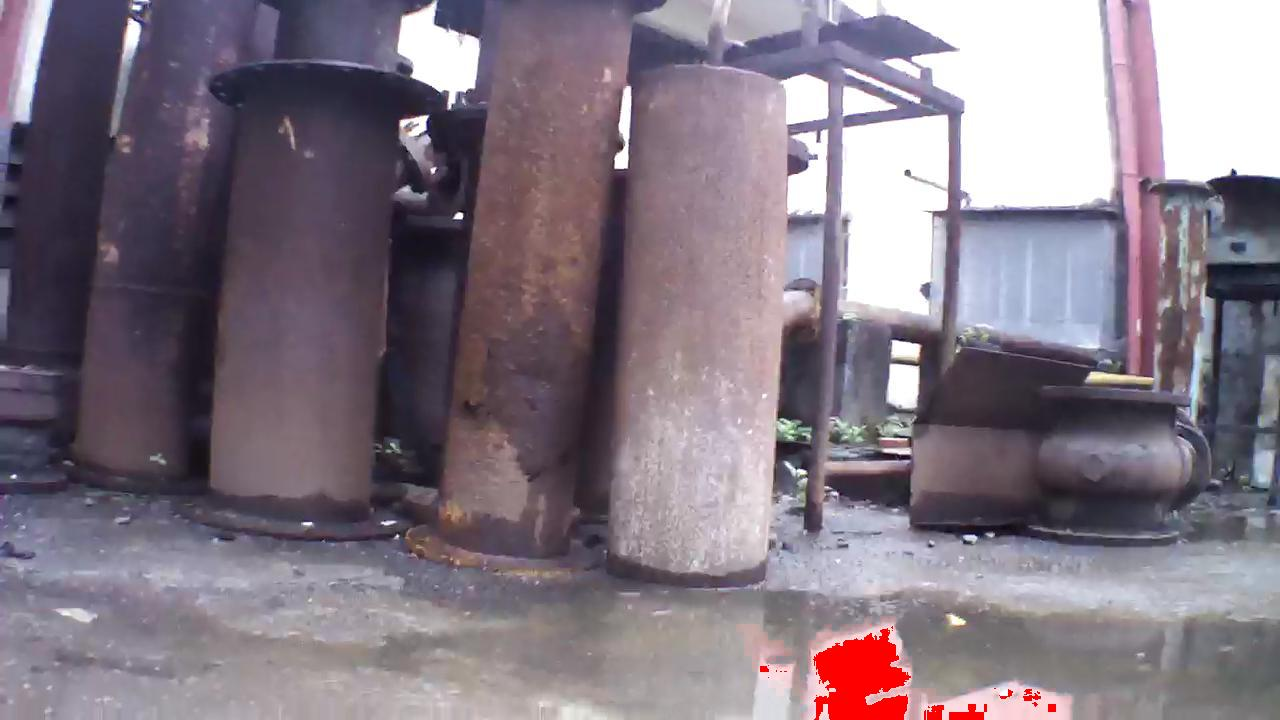
\includegraphics[width=0.32\linewidth]{stagnantWater/results/dataset_83/output_130}

  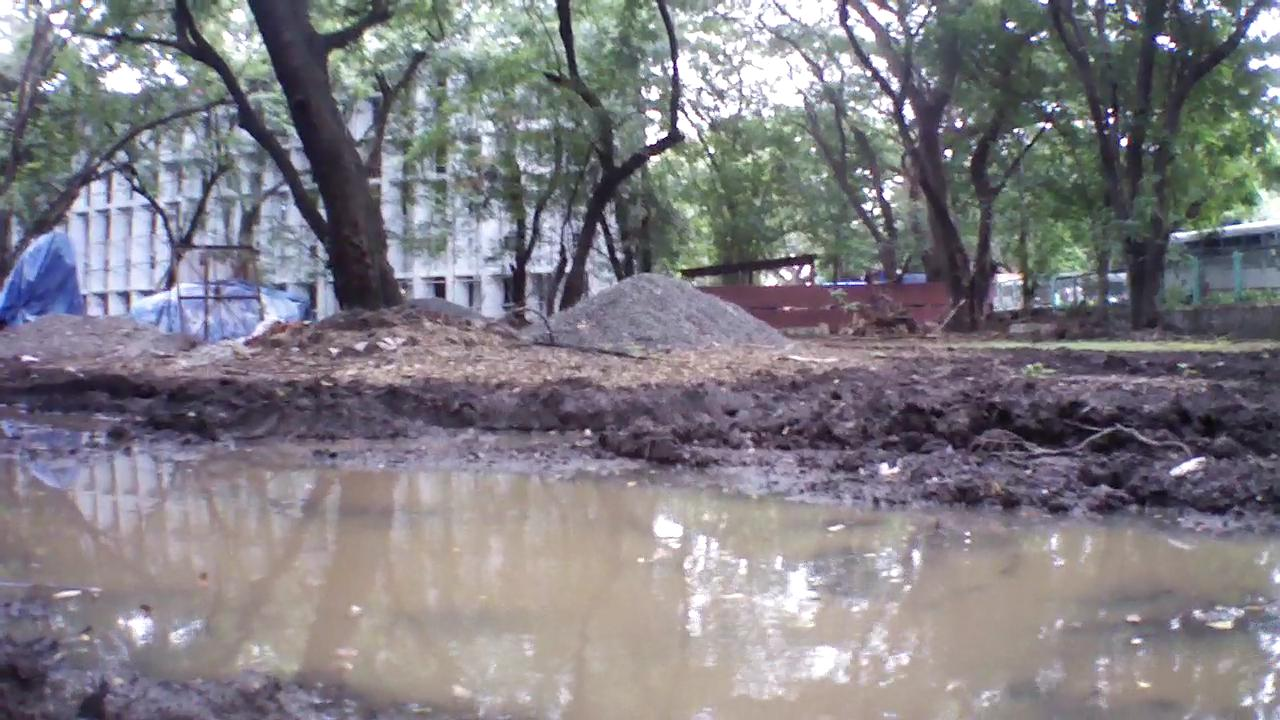
\includegraphics[width=0.32\linewidth]{stagnantWater/results/dataset_63full/IMG_PAIR_102_1} \hfill
  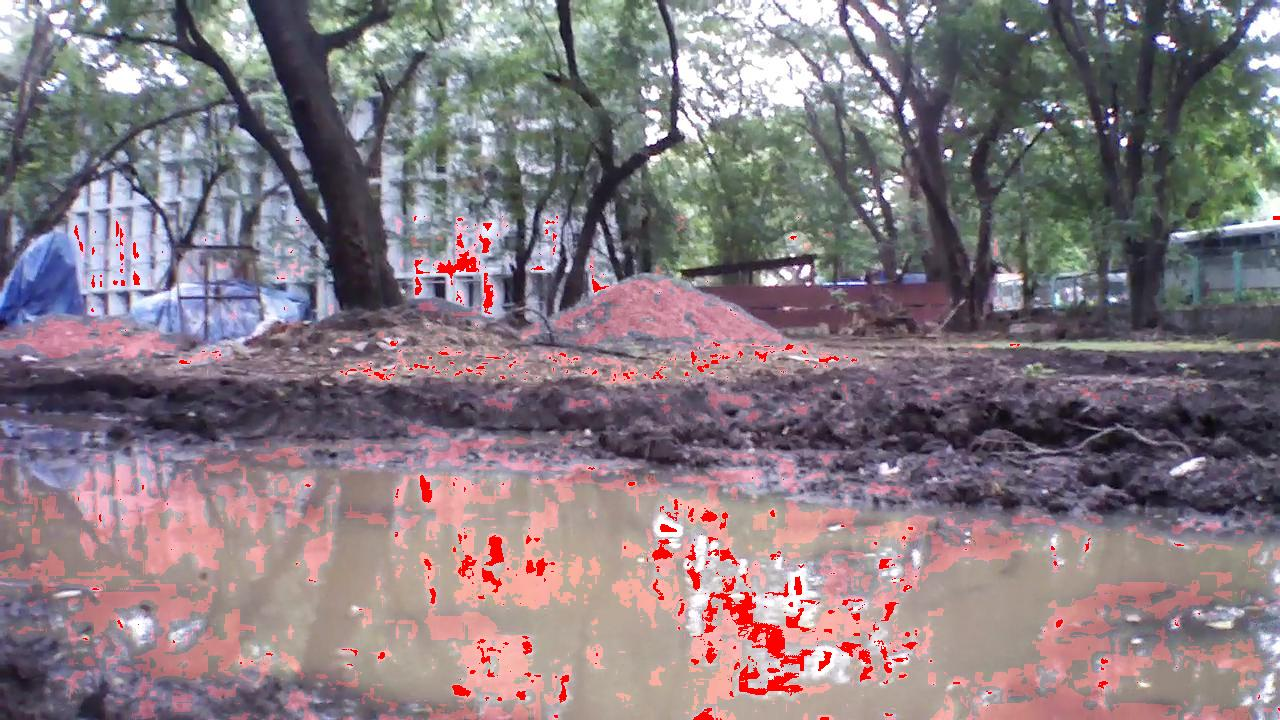
\includegraphics[width=0.32\linewidth]{stagnantWater/results/dataset_63full/output_102_jpl2} \hfill
  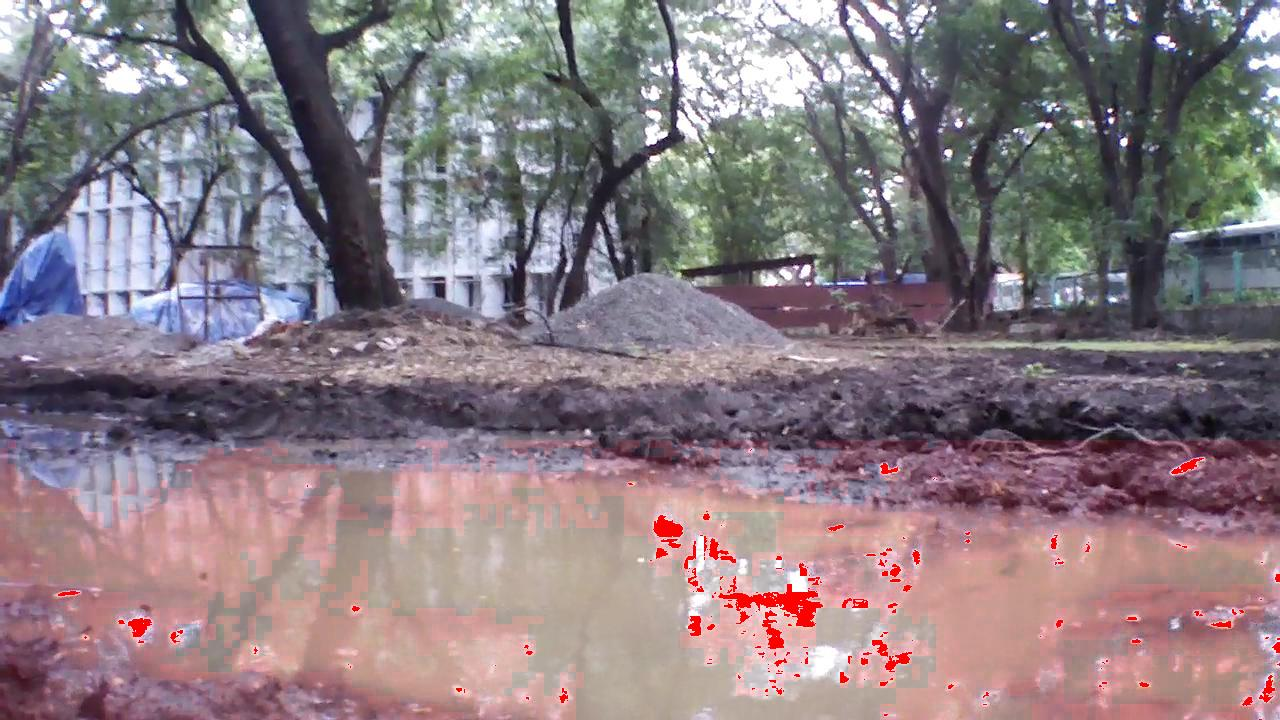
\includegraphics[width=0.32\linewidth]{stagnantWater/results/dataset_63full/output_102}
  	
  \caption{Comparison of proposed method with \cite{rankin2004daytime}. Confidence in detection is indicated by red hue in the output image. 
So, darker the red tinge, higher the confidence in detected water regions. \textbf{Left:} Original Image,
    \textbf{Middle:} Output of \cite{rankin2004daytime} \textbf{Right:}
    Proposed method. It can be seen that \cite{rankin2004daytime} is unable to
    detect textured puddle regions. Also, several false positives are
    seen to appear in the middle row.  Our method is sedate and
    sufficient to alert health workers.}
\label{fig:comparison}
\end{figure}

\newpage
\bibliographystyle{plain}
\bibliography{egbib}
\end{document}
